\subsection{\texorpdfstring{\(B_{l}\) 型根系（\(l \geqslant 2\)）}{B\_l 型根系 (l >= 2)}}

\begin{enumerate}
\def\labelenumi{(\Roman{enumi})}
\item
  我们考虑 \(L_{0}\)，它是 V = \(R^{l}\)（第 4 号）中的群。令 R 为由满足 \(\alpha \in L_{0}\) 且 \((\alpha|\alpha) = 1\) 或 \((\alpha|\alpha) = 2\) 的元素所成的集合，换言之，是由向量 \(\pm\varepsilon_{i}\)（\(1 \leqslant i \leqslant l\)）和 \(\pm\varepsilon_{i} \pm \varepsilon_{j}\)（\(1 \leqslant i < j \leqslant l\)）组成的集合。显然，R 生成 V，且 \(2(\alpha|\beta)/(\alpha|\alpha) \in \mathbf{Z}\) 对所有 \(\alpha, \beta \in R\) 成立。因此 R 是 V 中的约化根系（第 4 号）。根的数目为 \(n = 2l + 4\frac{l(l-1)}{2} = 2l^{2}\)。
\item
  置
\end{enumerate}

\[
\alpha_ {1} = \varepsilon_ {1} - \varepsilon_ {2}, \alpha_ {2} = \varepsilon_ {2} - \varepsilon_ {3}, \dots , \alpha_ {l - 1} = \varepsilon_ {l - 1} - \varepsilon_ {l}, \alpha_ {l} = \varepsilon_ {l}.
\]

于是

\[
\begin{array}{c} \varepsilon_ {i} = \alpha_ {i} + \alpha_ {i + 1} + \dots + \alpha_ {l} \quad (1 \leqslant i \leqslant l) \\ \varepsilon_ {i} + \varepsilon_ {j} = (\alpha_ {i} + \alpha_ {i + 1} + \dots + \alpha_ {l}) + (\alpha_ {j} + \alpha_ {j + 1} + \dots + \alpha_ {l}) (1 \leqslant i <   j \leqslant l) \\ \varepsilon_ {i} - \varepsilon_ {j} = \alpha_ {i} + \alpha_ {i + 1} + \dots + \alpha_ {j - 1} \quad (1 \leqslant i <   j \leqslant l). \end{array}
\]

因此 \((\alpha_{1},\alpha_{2},\ldots ,\alpha_{l})\) 是 R 的一组基（第 1 节，第 7 号，命题 20 的推论 3）。此外，\(\| \alpha_{i}\|^{2} = 2\) 对 \(i < l\) 成立，\(\| \alpha_l\| ^2 = 1\)，\((\alpha_i|\alpha_{i + 1}) = -1\) 对 \(1\leqslant i\leqslant l - 1\) 成立，\((\alpha_i|\alpha_j) = 0\) 对 \(j > i + 1\) 成立：因此 R 的 Dynkin 图为 \(\mathbf{B}_l\) 型，这表明 R 不可约。正根是 \(\varepsilon_{i}\) 以及 \(\varepsilon_{i}\pm \varepsilon_{j}\)（\(i < j\)）。

\begin{enumerate}
\def\labelenumi{(\Roman{enumi})}
\setcounter{enumi}{2}
\tightlist
\item
  根据第五章第 6 节第 2 号定理 1 (ii)。
\end{enumerate}

\[
h = n / l = 2 l.
\]

\begin{enumerate}
\def\labelenumi{(\Roman{enumi})}
\setcounter{enumi}{3}
\tightlist
\item
  令 \(\tilde{\alpha} = \varepsilon_{1} + \varepsilon_{2} = \alpha_{1} + 2\alpha_{2} + 2\alpha_{3} + \cdots + 2\alpha_{l}\)，这是一个根。它相对于基 \((\alpha_{i})\) 的坐标之和为 2l - 1 = h - 1。根据第 1 节第 11 号命题 31，\(\tilde{\alpha}\) 是 R 的最高根。有 \((\tilde{\alpha}| \alpha_{i}) = 0\) 对 \(i \neq 2\) 成立，且 \((\tilde{\alpha}| \alpha_{2}) = 1\)。由于 \(\alpha_{2}\) 的长度分别为 1 和 \(\sqrt{2}\)，对应于 l = 2 和 \(l \geqslant 3\)，R 的完备 Dynkin 图如下：
\end{enumerate}

\[
\text { for } l = 2 \quad \alpha_ {2} \alpha_ {1}
\]

\pandocbounded{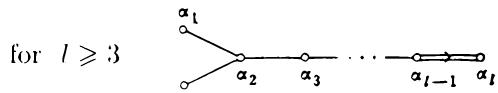
\includegraphics[keepaspectratio]{images/part002_79c781e2.jpg}}

\begin{enumerate}
\def\labelenumi{(\Alph{enumi})}
\setcounter{enumi}{21}
\tightlist
\item
  公式 \(\alpha^{\prime} = \frac{2\alpha}{(\alpha|\alpha)}\) 给出 \(R^{\prime}\) 的向量集：\(\pm 2\varepsilon_{i}\)（\(1 \leqslant i \leqslant l\)）以及 \(\pm \varepsilon_{i} \pm \varepsilon_{j}\)（\(1 \leqslant i < j \leqslant l\)）。\(R^{\prime}\) 的 Dynkin 图按照第 2 号所述过程由 \(R\) 的 Dynkin 图得到，并可见 \(R^{\prime}\) 为 \(C_{l}\) 型。
\end{enumerate}

有 \(4l - 2\) 个根不与 \(\beta = \varepsilon_1\) 正交，即 \(\pm \varepsilon_1\) 以及 \(\pm \varepsilon_1 \pm \varepsilon_j\)（\(2 \leqslant j \leqslant l\)）；对于每个这样的根 \(\alpha\)，\(n(\alpha, \beta) = \pm 2\)。第 1 节第 12 号的公式 (17) 表明，对于 \(\Phi_{\mathrm{R}}\)，\(\beta\) 的长度平方为 \((4l - 2)^{-1}\)；因此 \(\Phi_{\mathrm{R}}(x, y) = (x|y)/(4l - 2)\)。在 \(x = y = \beta\) 的情形应用第 1 节第 12 号的公式 (18)。这给出

\[
2 + \frac {1}{4} (4 l - 4) = \gamma (R) \frac {1}{4 l - 2}
\]

从而 \(\gamma(R) = (l + 1)(4l - 2)\)。

\begin{enumerate}
\def\labelenumi{(\Roman{enumi})}
\setcounter{enumi}{5}
\tightlist
\item
  基本权 \(\omega_{i}\)（\(1 \leqslant i \leqslant l\)）满足 \((\omega_{i}|\alpha_{j}) = \delta_{ij}\)，容易计算，得到
\end{enumerate}

\[
\begin{array}{l} \omega_ {i} = \varepsilon_ {1} + \varepsilon_ {2} + \dots + \varepsilon_ {i} \\ \qquad = \alpha_ {1} + 2 \alpha_ {2} + \dots + (i - 1) \alpha_ {i - 1} + i (\alpha_ {1} + \alpha_ {i + 1} + \dots + \alpha_ {l}) (i <   l) \\ \omega_ {l} = \frac {1}{2} (\varepsilon_ {1} + \varepsilon_ {2} + \dots + \varepsilon_ {l}) = \frac {1}{2} (\alpha_ {1} + 2 \alpha_ {2} + \dots + l \alpha_ {l}). \end{array}
\]

\begin{enumerate}
\def\labelenumi{(\Roman{enumi})}
\setcounter{enumi}{6}
\tightlist
\item
  正根之和为
\end{enumerate}

\[
\begin{array}{l} 2 \rho = (2 l - 1) \varepsilon_ {1} + (2 l - 3) \varepsilon_ {2} + \dots + 3 \varepsilon_ {l - 1} + \varepsilon_ {l} \\ = (2 l - 1) \alpha_ {1} + 2 (2 l - 2) \alpha_ {2} + \dots + i (2 l - i) \alpha_ {i} + \dots + l ^ {2} \alpha_ {l}. \end{array}
\]

\begin{enumerate}
\def\labelenumi{(\Roman{enumi})}
\setcounter{enumi}{7}
\item
  有 \(Q(R) = L_{0}\)（第 4 号），且 \(P(R)\) 由 \(Q(R)\) 和 \(\omega_{l}\) 生成，故等于 \(L_{2}\)（第 4 号）。因此，\(P(R)/Q(R)\) 同构于 Z/2Z，连接指标等于 2。
\item
  以及 (X) 在 \(R^{l}\) 中，正交反射 \(s_{\varepsilon_{i}-\varepsilon_{j}}\)（\(i \neq j\)）交换 \(\varepsilon_{i}\) 和 \(\varepsilon_{j}\)，并在指标 k 异于 i 和 j 时保持 \(\varepsilon_{k}\) 不变。\(s_{\varepsilon_{i}-\varepsilon_{j}}\) 生成一个群 \(G_{1}\)，它同构于对称群 \(S_{l}\)。正交反射 \(s_{\varepsilon_{i}}\) 将 \(\varepsilon_{i}\) 变为 \(-\varepsilon_{i}\)，并在指标 k 异于 i 时保持 \(\varepsilon_{k}\) 不变。\(s_{\varepsilon_{i}}\) 生成一个群 \(G_{2}\)，它同构于 \((\mathbf{Z}/2\mathbf{Z})^{l}\)。韦伊群 W(R) 由 \(G_{1}\) 和 \(G_{2}\) 生成，且 \(G_{2}\) 是 W(R) 的正规子群，所以 W(R) 同构于 \(S_{l}\) 与 \((\mathbf{Z}/2\mathbf{Z})^{l}\) 的半直积。因此它的阶为 \(2^{l}\cdot l!\)。
\end{enumerate}

对称代数 \(\mathbf{S}(\mathbf{R}^{l})\) 可典范地与多项式函数代数 \(\mathrm{P}(\xi_{1},\ldots,\xi_{l})\) 认同，后者定义在 \(R^{l}\) 上。要使这样的多项式在 \(\mathrm{W}(\mathrm{R})\) 下不变，首先必须有

\[
P \left(\xi_ {1}. \xi_ {2}. \dots ., \xi_ {l}\right) = P \left(\pm \xi_ {1}. \pm \xi_ {2}. \dots ., \pm \xi_ {l}\right)
\]

对右端的符号作任意选择均成立，从而

\[
\mathrm{P} \left(\xi_ {1}, \dots , \xi_ {l}\right) = \mathrm{Q} \left(\xi_ {1} ^ {2}, \dots , \xi_ {l} ^ {2}\right)
\]

其中 Q 是多项式，并且 Q 还是对称多项式；这些条件也是充分的。因此（《代数》第五章附录 I），\(\mathbf{S}(\mathbf{R}^{l})^{\mathrm{W}(\mathbb{R})}\) 是由以下 l 个多项式函数生成的代数

\[
t _ {i} = \sum_ {\tau \in \mathfrak {S} _ {l}} \xi_ {\tau (1)} ^ {2} \xi_ {\tau (2)} ^ {2} \dots \xi_ {\tau (l)} ^ {2} \quad (1 \leqslant i \leqslant l).
\]

此外，\(\mathbf{R}\) 上的 \(\mathbf{S}(\mathbf{R}^l)^{\mathrm{W(R)}}\) 的分式域的超越次数为 \(l\)，所以 \(t_i\) 代数独立。由于 \(t_i\) 的次数为 \(2,4,\ldots ,2l\)，我们得到 \(\mathrm{W(R)}\) 的指数（第五章第 6 节第 3 号命题 3）为：

\[
1, 3, 5, \dots , 2 l - 1.
\]

\begin{enumerate}
\def\labelenumi{(\Roman{enumi})}
\setcounter{enumi}{10}
\item
  Dynkin 图的唯一自同构是恒等元。因此，\(A(R) = W(R)\) 且 \(-1 \in W(R)\)。由于 -1 将 B 变为 -B，我们得到 \(w_{0} = -1\)。
\item
  群 \(P(R^{\prime})/Q(R^{\prime})\) 是 \(P(R)/Q(R)\) 的对偶，因而同构于 Z/2Z。其非平凡元置换对应于 \(\alpha_{0}\) 和 \(\alpha_{1}\) 的顶点，并固定其他顶点。
\end{enumerate}
% semantic-fragments: legacy-input-seam
\relax{}
